\documentclass[11pt]{article}
\usepackage[utf8]{inputenc}
\usepackage{amsmath, amssymb}
\usepackage{geometry}
\usepackage{listings}
\usepackage{xcolor}
\usepackage{graphicx}
\usepackage{tabularx}
\usepackage{booktabs}
\usepackage{hyperref}
\usepackage{wrapfig}
\usepackage{subcaption}

\geometry{a4paper, margin=1in}

\definecolor{codegray}{rgb}{0.5,0.5,0.5}
\definecolor{codepurple}{rgb}{0.58,0,0.82}
\definecolor{backcolour}{rgb}{0.95,0.95,0.92}

\lstset{
    language=Python,
    backgroundcolor=\color{backcolour},
    commentstyle=\color{codegray},
    keywordstyle=\color{magenta},
    stringstyle=\color{codepurple},
    basicstyle=\ttfamily\small,
    breaklines=true,
    showstringspaces=false
}

\title{Physics Lab: Electric Field Lines Tracing \\ \large Problem Set \& Implementation Guide}
\author{Scientific Programming Course}
\date{2026}

\begin{document}

%\maketitle

\section*{Problem 1: Electric Field Direction}

\subsubsection*{Mathematical part}
\begin{wrapfigure}{r}{0.4\textwidth}
 \centering
 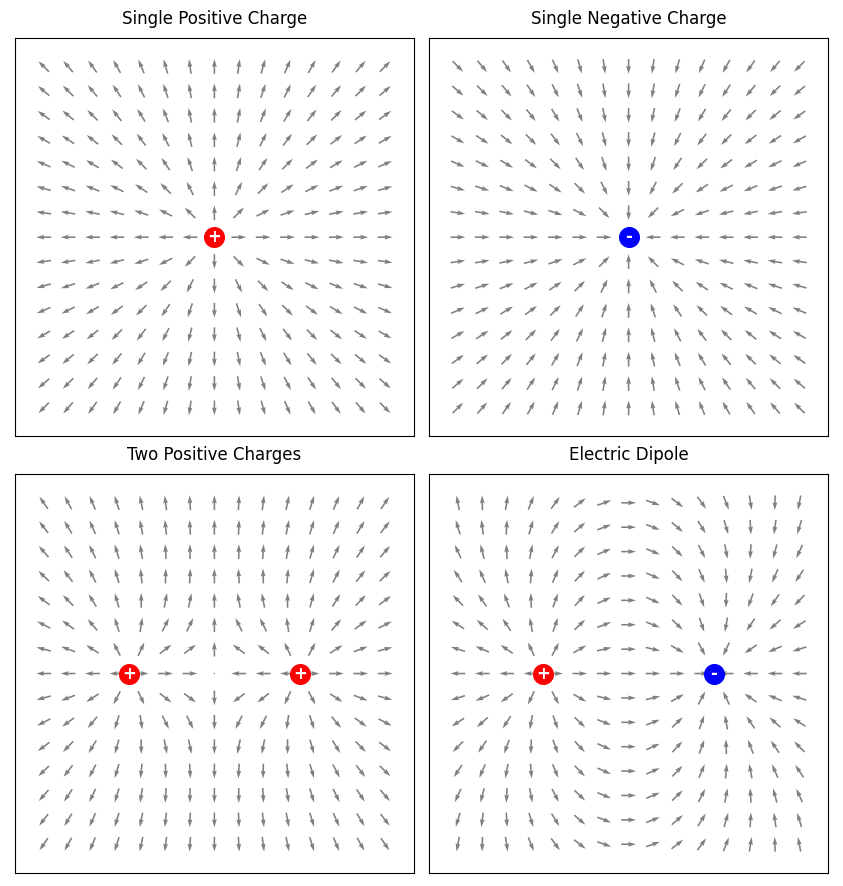
\includegraphics[width=0.5\textwidth]{Electric_Field_Direction}
 \caption{Electric field directions.}
 \label{fig_electric}
 \vspace{-3cm}
\end{wrapfigure}

\textbf{Given:} An observation point in space $\mathbf{r}$, and a set of $N$ point charges with positions $\mathbf{R}_i$ and charge values $Q_i$. \\
\textbf{Derive:} The normalized direction vector of the net electric field $\hat{\vec{E}}$ at the observation point $\mathbf{r}$. \\
\textbf{Hint:} Use Coulomb's law and the superposition principle:
$$
\vec{E}(\mathbf{r}) = \sum_{i=1}^{N} \frac{Q_i}{|\mathbf{r} - \mathbf{R}_i|^3} (\mathbf{r} - \mathbf{R}_i).
$$
\textbf{Do not forget} to normalize the resulting vector. To prevent division by zero, cap the squared distances using the predefined \lstinline|CORE_RADIUS_SQ| constant.


\subsubsection*{Implementation part}
\textbf{Implement:} a function
\begin{lstlisting}
calc_E_dir(pt,
           charges_positions,
           charges_values)
\end{lstlisting}
that returns the normalized direction $\hat{\vec{E}}$ as a \lstinline|numpy.array|.
\begin{center}
\renewcommand{\arraystretch}{2.0}
\begin{tabular}{r | c | c | c | c}
\toprule
\textbf{Math Symbol} & $\mathbf{r}$ & $\mathbf{R}$ & $\mathbf{Q}$ & $\hat{E}$ \\ \midrule
\textbf{Argument} & \lstinline|pt| & \lstinline|charges_positions| & \lstinline|charges_values| & \lstinline|return| \\ \midrule
\textbf{Type} & \lstinline|np.array| & \lstinline|np.array| & \lstinline|np.array| & \lstinline|np.array| \\
\bottomrule
\end{tabular}
\end{center}
\textbf{Test:} Launch the \lstinline|test_calc_E_dir.py| file. If results are correct you should see a familiar picture~\ref{fig_electric}.



\vspace{1cm}

\section*{Problem 2: Field Line Trajectory (RK2 Midpoint)}

\subsubsection*{Mathematical part}
\textbf{Given:} A starting point for a streamline $\mathbf{r}_0$, the sign of the source charge $s$, and the spatial configuration $\mathbf{R}_i$ of all charges $\mathbf{Q}_i$. \\
\textbf{Derive:} The iterative coordinates of the streamline $\mathbf{r}_{i+1}$ as a function of $\mathbf{r}_i$ utilizing the 2nd-Order Runge-Kutta (Midpoint) method. \\
\textbf{Hint:} For each step of size $h$, first calculate the direction of step $\hat{\vec{E}}(\mathbf{r}_i) s$. Instead of doing the full step in this direction, scout the midpoint (do half-step $h/2$) and find electric field direction there $\hat{\vec{E}}_{\text{midpoint}}$, then use this direction to make the full step $h$ from $\mathbf{r}_i$.
The integration \textbf{must stop early} if the line enters the \lstinline|CORE_RADIUS_SQ| of any charge. \\

\subsubsection*{Implementation part}
\textbf{Implement:} a function
\begin{lstlisting}
propagate_trajectory(trajectory, current_charge_sign,
                     charges_positions, charges_values,
                     max_steps, step_size)
\end{lstlisting}
that modifies the \lstinline|trajectory| array \textbf{in-place} and returns the \textbf{total number of steps taken}. Note that the initial point is already in the \lstinline|trajectory[0]| so you can just extract it \lstinline|current_point = trajectory[0]|
\begin{center}
\renewcommand{\arraystretch}{2.0}
\begin{tabular}{|>{\centering\arraybackslash}p{2.5cm} | c | c | c | c | c |}
\toprule
$\mathbf{r}_i$ & $s$ & $\mathbf{R}$ & $\mathbf{Q}$ & $h$ & $N_{steps}$ \\ \midrule
\lstinline|trajectory|  & \lstinline|current_charge_sign| & \lstinline|charges_positions| & \lstinline|charges_values| & \lstinline|step_size| & \lstinline|return| \\ \midrule
\lstinline|np.array| \footnotesize\textcolor{red}{modify in place} & \lstinline|float| & \lstinline|np.array| & \lstinline|np.array| & \lstinline|float| & \lstinline|int| \\
\bottomrule
\end{tabular}
\end{center}
\textbf{Test 1:} Launch the \lstinline|test_propagate_trajectory.py| file. If results are correct you should see a familiar picture~\ref{fig_lines}.
%\begin{figure}[ht]
% \centering
% 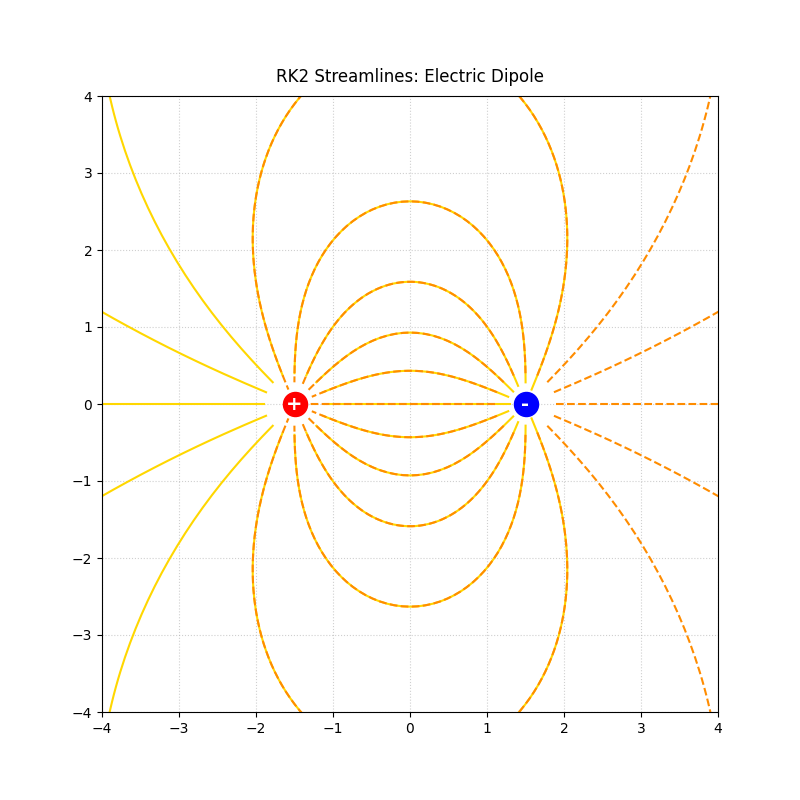
\includegraphics[width=0.7\textwidth]{Field_Lines}
% \caption{Electric field lines.}
% \label{fig_lines}
%\end{figure}
\begin{figure}[htbp]
    \centering

    % --- Figure A ---
    \begin{subfigure}[b]{0.45\textwidth}
        \centering
        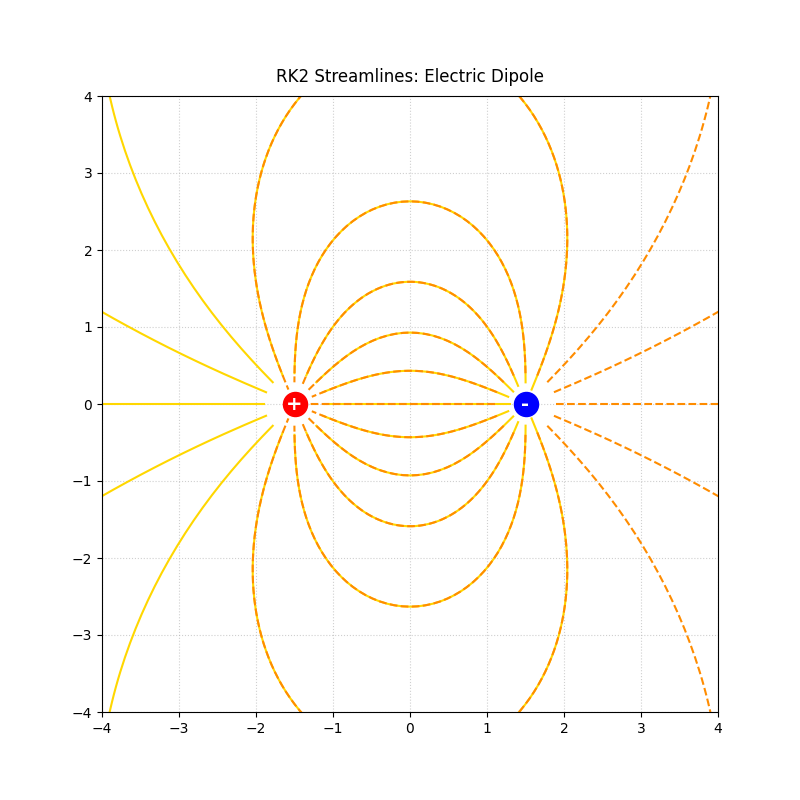
\includegraphics[width=\textwidth]{Field_Lines}
        \caption{Electric field lines, 2D case.}
        \label{fig_lines}
    \end{subfigure}
    \hfill % <--- This pushes them apart so they don't overlap
    % --- Figure B ---
    \begin{subfigure}[b]{0.45\textwidth}
        \centering
        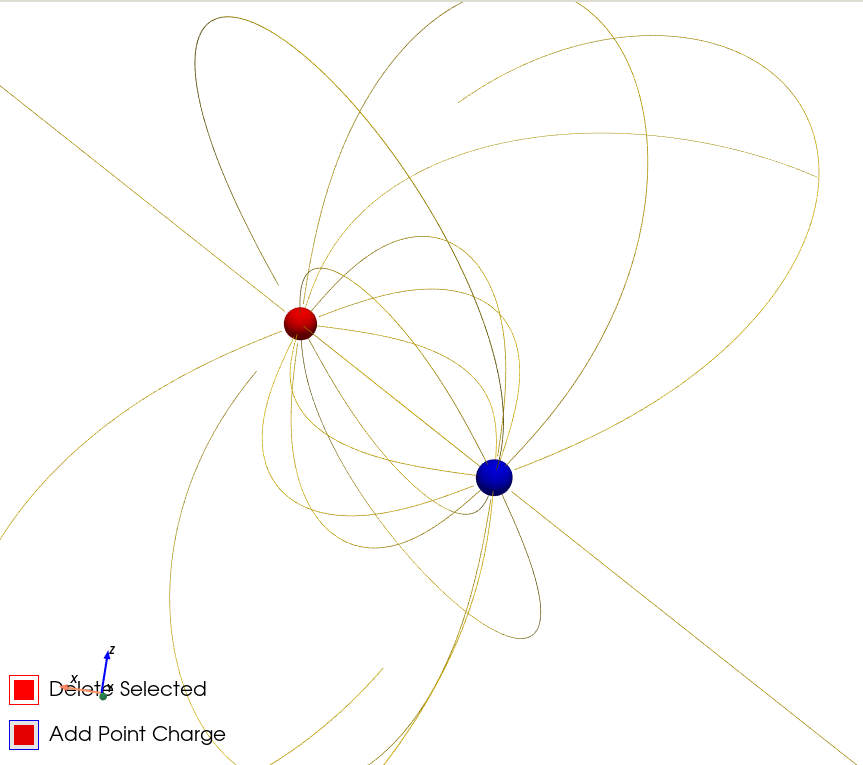
\includegraphics[width=\textwidth]{two_charges_3d}
        \caption{Electric field lines, 3D case.}
        \label{fig_lines_3d}
    \end{subfigure}

    \caption{Runge-Kutta 2 integration steps for an electric dipole.}
    \label{fig:rk2_main}
\end{figure}
\par\noindent\textbf{Test 2:} Launch the \lstinline|editor.py| file. Press the "Add Point Charge" button in the visual debugger window. Move the charge using Shift+Drag. Change the charge magnitude using the slider. If implemented correctly, smooth, continuous field lines will draw instantly and warp dynamically as you interact with the UI. Try building a dipole, it should look like figure~\ref{fig_lines_3d}.

\end{document}
